\documentclass{beamer}
\usepackage{textpos}
\setlength{\TPHorizModule}{1cm} % Horizontale Einheit
\setlength{\TPVertModule}{1cm} % Vertikale Einheit
\usepackage{lmodern}
\usepackage{xcolor}
\usepackage{algpseudocode}
\usepackage{amsmath}
\usepackage{tcolorbox}
\usepackage{tikz}
\usepackage{adjustbox}
\usepackage{setspace}
\usepackage{caption}
\usepackage[font={color=black}]{subcaption}
\usepackage{ellipsis}
\usetikzlibrary{decorations.pathmorphing,calc}
\usetikzlibrary{decorations.pathreplacing}
\usetikzlibrary{positioning}
\usepackage{chemarrow}
\usepackage{slashbox}
\usepackage[ruled,vlined,linesnumbered]{algorithm2e}
\usepackage{siunitx}
\usepackage{relsize}
\usepackage{epstopdf}
\usepackage{3dplot}
\usepackage{threeparttable}
\usetikzlibrary{fit}
\usepackage[utf8]{inputenc}
\usepackage[upright]{fourier}
\usetikzlibrary{matrix,arrows,decorations.pathmorphing}
\usepackage{xparse}
\usepackage[nomessages]{fp}% http://ctan.org/pkg/fp
\usetikzlibrary{calc}
\usepackage{breqn} %for dmath
\usepackage{hyperref} 
\usepackage{arydshln}
\usetikzlibrary{shapes,fit}
\definecolor{univred}{rgb}{0.7, 0.0, 0.0}
\definecolor{drkgreen}{rgb}{0,0.26,0.15}
\definecolor{aureolin}{rgb}{0.99,0.93,0.0}
\DeclareMathOperator*{\argmax}{argmax}
%
%
\newcolumntype{C}[1]{>{\centering\let\newline\\\arraybackslash\hspace{0pt}}m{#1}}
\setbeamertemplate{background canvas}{%
    {\color{univred}\noindent\makebox[\paperwidth]{\rule{\paperwidth}{2.5ex}}
}}
\setbeamertemplate{frametitle}{\color{black}\bfseries\vskip2ex\insertframetitle\par\vskip-6pt\hrulefill}
\addtobeamertemplate{frametitle}{}{%
%CMU logo in header
    \begin{textblock*}{100mm}(0.87\textwidth,-1.425cm)
        \includegraphics[height=1.5cm,width=1.9cm,keepaspectratio]{cm_logo}
    \end{textblock*}
%ECE logo in footer
    \begin{textblock*}{10mm}(-.8cm,7.5cm)
        \includegraphics[height=2cm,width=2.5cm,keepaspectratio]{ece}
    \end{textblock*}
}
\addtobeamertemplate{footnote}{}{\vspace{2ex}}
\setbeamercolor*{item}{fg=black}
\setbeamertemplate{footline}[page number]{}
\setbeamercolor{page number in head/foot}{fg=univred}
\def\HiLi{\leavevmode\rlap{\hbox to \hsize{\color{green!50}\leaders\hrule height .8\baselineskip depth .5ex\hfill}}}
\title{\color{univred} A Comparison of Antenna Placement Algorithms}
\author{Abhinav Jauhri}
\date{\today}
\begin{document}
\begin{frame}
    \color{univred}
    \titlepage
\end{frame}

\begin{frame}{Outline of this talk}
    \begin{itemize}
        \setlength\itemsep{2em}
        \item Part 1: Introduction to the antenna placement problem
        \item Part 2: Description of stochastic algorithms, and formulation of an instance of antenna placment problem
        \item Part 3: Results of our experiments
    \end{itemize}
\end{frame}

\begin{frame}{\null}
    \begin{tcolorbox}[colback=green!5]
        \centering\Huge
        Part 1: Introduction to the antenna placement problem
    \end{tcolorbox}
\end{frame}

\begin{frame}{Antenna Placement Problem}
    \centering
    \begin{columns}
        \column{0.33\linewidth}
        \only<1->{
            \begin{textblock}{3}(0.2,-2.8) Given, platform \end{textblock}
            \begin{textblock}{3}(0.2,-0.9)
                \begin{figure}
                    \includegraphics[trim=175 165 140 165, clip, scale=0.4]{../paper/FIG/tc_1_platform}
                \end{figure}\end{textblock}
        }
        \only<2->{
            \begin{textblock}{3}(-1,2)\textbf{Problem:} find best antenna placements \end{textblock}
            \begin{textblock}{3}(2.5,0.5)
                \begin{figure}
                    \includegraphics[trim=170 165 70 15, clip, scale=0.4]{../paper/FIG/tc_11_figure}
                \end{figure}\end{textblock}
        }
        \column{0.33\linewidth}
        \only<1->{
            \begin{textblock}{6}(-1.5,-2.8) + \end{textblock}
            \begin{textblock}{6}(-0.7,-2.8) allowable placements of antennas \end{textblock}
            \begin{textblock}{3}(-0.2,-2.9)
                \begin{figure}
                    \includegraphics[trim=170 165 70 15, clip, scale=0.4]{../paper/FIG/tc_1_figure2}
                \end{figure}\end{textblock}
        }
    \end{columns}
\end{frame}

\begin{frame}[t]{Antenna Placement Problem}
    Given:
\begin{itemize} \itemsep1.5em
        \item platform $P$ with its surface gridded such that end points represent possible antenna placements
        \item set of  $m~(m > 1)$ antennas $A = {A_1, A_2, \dots, A_m}$
        \item for each $A_i$, let $L_i$ denote the set of allowable placements $\in \mathbb R^3$ such that $\mid L_i \mid = n_i$ and $\forall i, n_i > 1$; $L_i = \{(x_{1}, y_{1}, z_{1}) \dots (x_{n_i}, y_{n_i}, z_{n_i})\}$
    \end{itemize}
    \vspace{10px}
    \centering\only{\textbf{Problem}: Find a set of $n$ optimal antenna placements on $P$}
\end{frame}

\begin{frame}{\null}
    \begin{tcolorbox}[colback=green!5]
        \centering
        Question: How is a good antenna placement quantified in the context of platform and other antennas?
    \end{tcolorbox}
\end{frame}

\begin{frame}[t]{Mutual Coupling}
    When two antennas are in proximity, and one is transmitting, the second will receive some of the transmitted energy.\\ \vspace{2mm}
    \begin{figure}\centering
        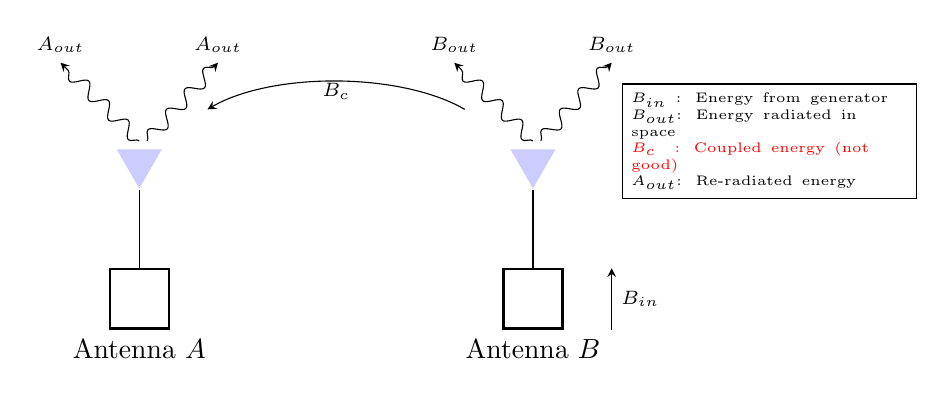
\begin{tikzpicture} [
                triangle/.style = {fill=blue!20, regular polygon, regular polygon sides=3 },
                node rotated/.style = {rotate=180},
                border rotated/.style = {shape border rotate=180}
            ]
            \node (b1) at (0, 1) [draw,thick,minimum width=.75cm,minimum height=.75cm, label=below:Antenna $A$] {}; 
            \node[triangle, border rotated, above=1cm of b1] (a1) {};
            \draw [-] (a1) -- (b1);
            \node (b2) at (5, 1) [draw,thick,minimum width=.75cm,minimum height=.75cm, label=below:Antenna $B$] {}; 
            \node[triangle, border rotated, above=1cm of b2] (a2) {};
            \draw [-] (a2) -- (b2);
            \draw [-stealth] ([xshift=1cm] b2.south) to node[right] {\scriptsize $B_{in}$} ([xshift=1cm] b2.north);
            \draw [stealth-, shorten <= 1cm, shorten >= 1cm] (a1.north) to[bend left] node {\scriptsize $B_c$} (a2.north);
            \draw [-stealth,decorate,decoration=snake] ([yshift=.1cm, xshift=.1cm] a1.north) -- (1,4) node[above] {\scriptsize $A_{out}$};
            \draw [-stealth,decorate,decoration=snake] ([yshift=.1cm] a1.north) -- (-1,4) node[above] {\scriptsize $A_{out}$};
            \draw [-stealth,decorate,decoration=snake] ([yshift=.1cm, xshift=.1cm] a2.north) -- (6,4) node[above] {\scriptsize $B_{out}$};
            \draw [-stealth,decorate,decoration=snake] ([yshift=.1cm] a2.north) -- (4,4) node[above] {\scriptsize $B_{out}$};
            \node[draw, text width=3.5cm] at (8,3) {\tiny $B_{in}~$:  Energy from generator\\$B_{out}$: Energy radiated in space\\{\color{red}$B_c~~$: Coupled energy (not good)}\\$A_{out}$: Re-radiated energy\\}; 
        \end{tikzpicture}
    \end{figure}
\end{frame}

\begin{frame}{Minimize Mutual Coupling}
    \begin{tcolorbox}[colback=green!5]
        \begin{equation}
            F_{MC} = \sum_{i=1}^{n-1}\sum_{j=i+1}^{n} CP(A_i, A_j),
        \end{equation}
    \end{tcolorbox}
    where
    \begin{itemize}
        \item $CP(\cdot)$ computes the coupling between two antennas via a simulator
        \item $i \neq j$
    \end{itemize}
    \vspace{2mm}
    \small\textit{Example:} If $n=3$, then $F_{MC} = CP(A_1, A_2) + CP(A_1, A_3) + CP(A_2, A_3)$
\end{frame}


\begin{frame}{Minimize Difference in Radiation Pattern}
    Pattern defines the ratio of energy radiated and input energy in a particular direction. For each antenna $A_i$:
    \begin{tcolorbox}[colback=green!5]
        \begin{equation} \label{eq:rp}
            F_{RP} = \sum_i^n\sum_{\theta}\sum_{\phi} 
            \left( FSG_i(\theta,\phi) - ISG_i(\theta,\phi) \right) ^2,
        \end{equation}
    \end{tcolorbox}
    where
    \begin{itemize}
            \small
        \item $\theta, \phi$ spherical coordinates
        \item $FSG(\cdot)$ returns free-space gain pattern  
        \item $ISG(\cdot)$ returns in-situ gain pattern
    \end{itemize}

    \tdplotsetmaincoords{60}{110}
    \pgfmathsetmacro{\rvec}{.8}
    \pgfmathsetmacro{\thetavec}{30}
    \pgfmathsetmacro{\phivec}{60}
    \hspace{.6\textwidth}
    \begin{tikzpicture}[scale=1.8,tdplot_main_coords]
        \tikzstyle{every node}=[font=\tiny]
        \coordinate (O) at (0,0,0);
        \tdplotsetcoord{P}{\rvec}{\thetavec}{\phivec}
        \draw[thick,->] (0,0,0) -- (1,0,0) node[anchor=north east]{$x$};
        \draw[thick,->] (0,0,0) -- (0,1,0) node[anchor=north west]{$y$};
        \draw[thick,->] (0,0,0) -- (0,0,1) node[anchor=south]{$z$};
        \draw[-stealth,color=red] (O) -- (P);
        \draw[dashed, color=red] (O) -- (Pxy);
        \draw[dashed, color=red] (P) -- (Pxy);
        \tdplotdrawarc{(O)}{0.2}{0}{\phivec}{anchor=north}{$\phi$}
        \tdplotsetthetaplanecoords{\phivec}
        \tdplotdrawarc[tdplot_rotated_coords]{(0,0,0)}{0.5}{0}{\thetavec}{anchor=south west}{$\theta$}
        \draw[dashed,tdplot_rotated_coords] (\rvec,0,0) arc (0:90:\rvec);
        \draw[dashed] (\rvec,0,0) arc (0:90:\rvec);
    \end{tikzpicture}
\end{frame}

\begin{frame}{Objective Function}
    Find a placement such that $F$ is minimal:
    \begin{tcolorbox}[colback=green!5]
        \begin{equation} \label{eq:optimal}
            F = \alpha F_{MC} + \beta F_{RP},
        \end{equation}
    \end{tcolorbox}
    where $\alpha + \beta = 1$
\end{frame}



\begin{frame}[t]{Contributions}
    \begin{itemize}
        \item Formulation of the antenna placement problem
        \item Evaluation of standard stochastic algorithms on a real-world problem
        \item Able to achieve global optimum with as low as 21\% evaluations of search space
    \end{itemize}
    \vspace{5mm}
\end{frame}


\begin{frame}{\null}
    \begin{tcolorbox}[colback=green!5]
        \centering\Huge
        Part 2: Stochastic Algorithms
    \end{tcolorbox}
\end{frame}
\begin{frame}[t]{Stochastic Algorithms}
    We will consider algorithms which rely on \textit{randomization} principle.
    \vspace{10px}
\begin{itemize} \itemsep1.5em
        \item Genetic Algorithm
        \item Evolutionary Strategy
        \item Simulated Annealing
        \item Hill Climbing
    \end{itemize}
\end{frame}

\begin{frame}[t]{Stochastic Algorithms: Mutation Operator}
    \begin{enumerate}
        \item From individual, select an antenna uniformly at random, let's say antenna 1:\par
            \begin{minipage}[t]{\linewidth}
                \centering
                \adjustbox{valign=t}{%
                    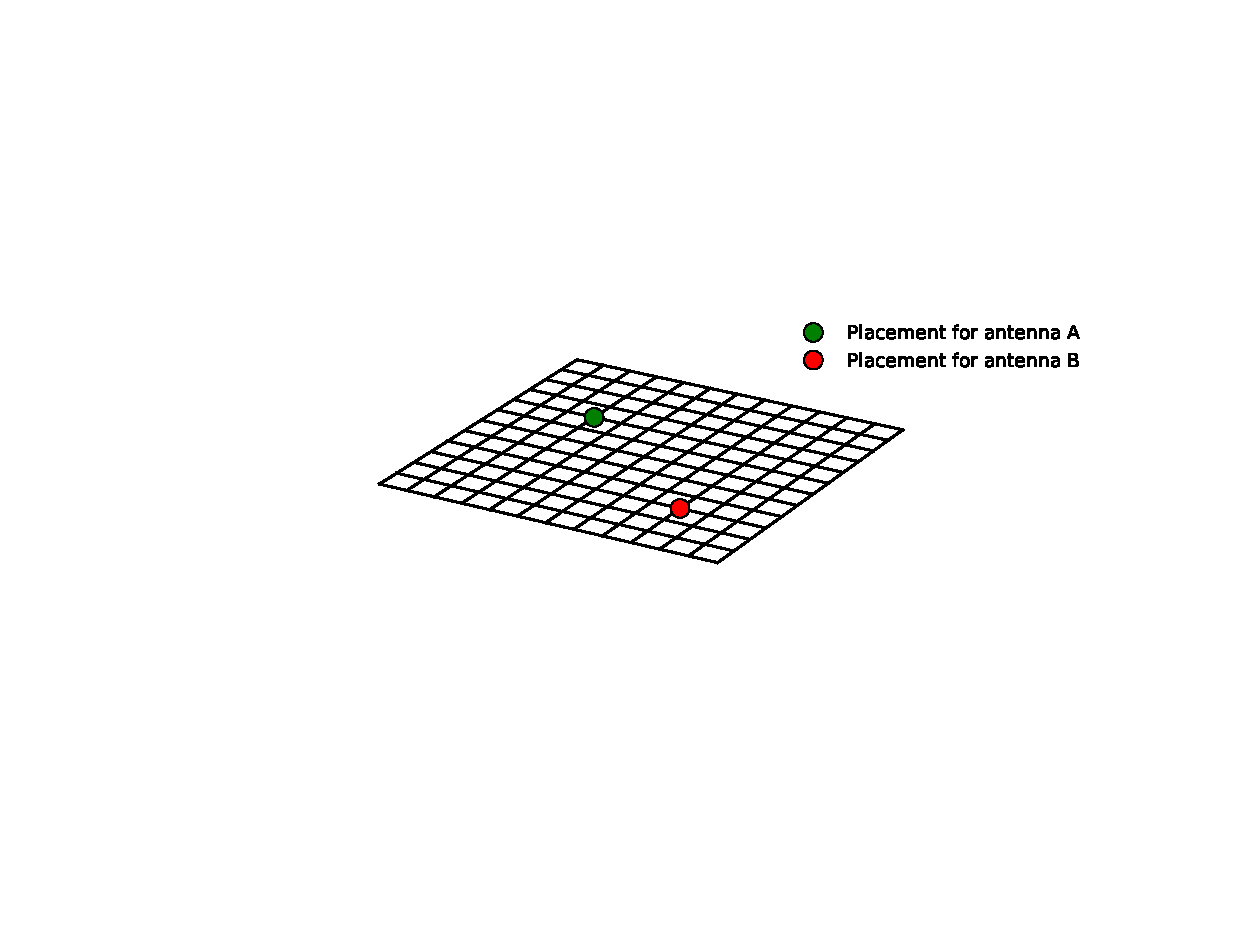
\includegraphics[trim=175 165 50 135, clip, scale=0.35]{../paper/FIG/tc1_mut1}
                }
            \end{minipage}
        \item For antenna 1, select any other placement:\par
            \begin{minipage}[t]{\linewidth}
                \centering
                \adjustbox{valign=t}{%
                    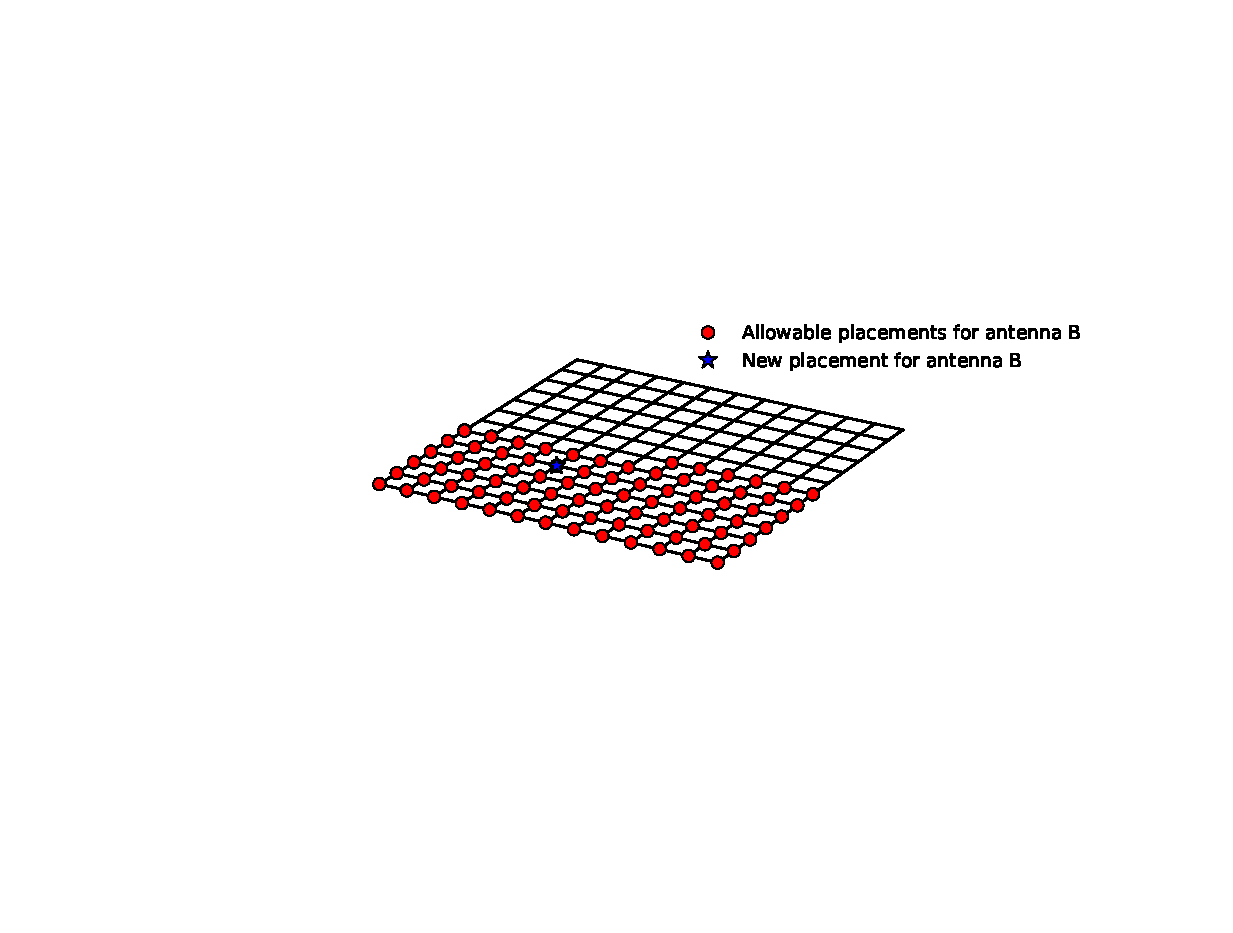
\includegraphics[trim=125 165 50 135, clip, scale=0.35]{../paper/FIG/tc1_mut2}
                }
            \end{minipage}
        \item Change position for antenna 1 in individual:\par
            \begin{minipage}[t]{\linewidth}
                \centering
                \adjustbox{valign=t}{%
                    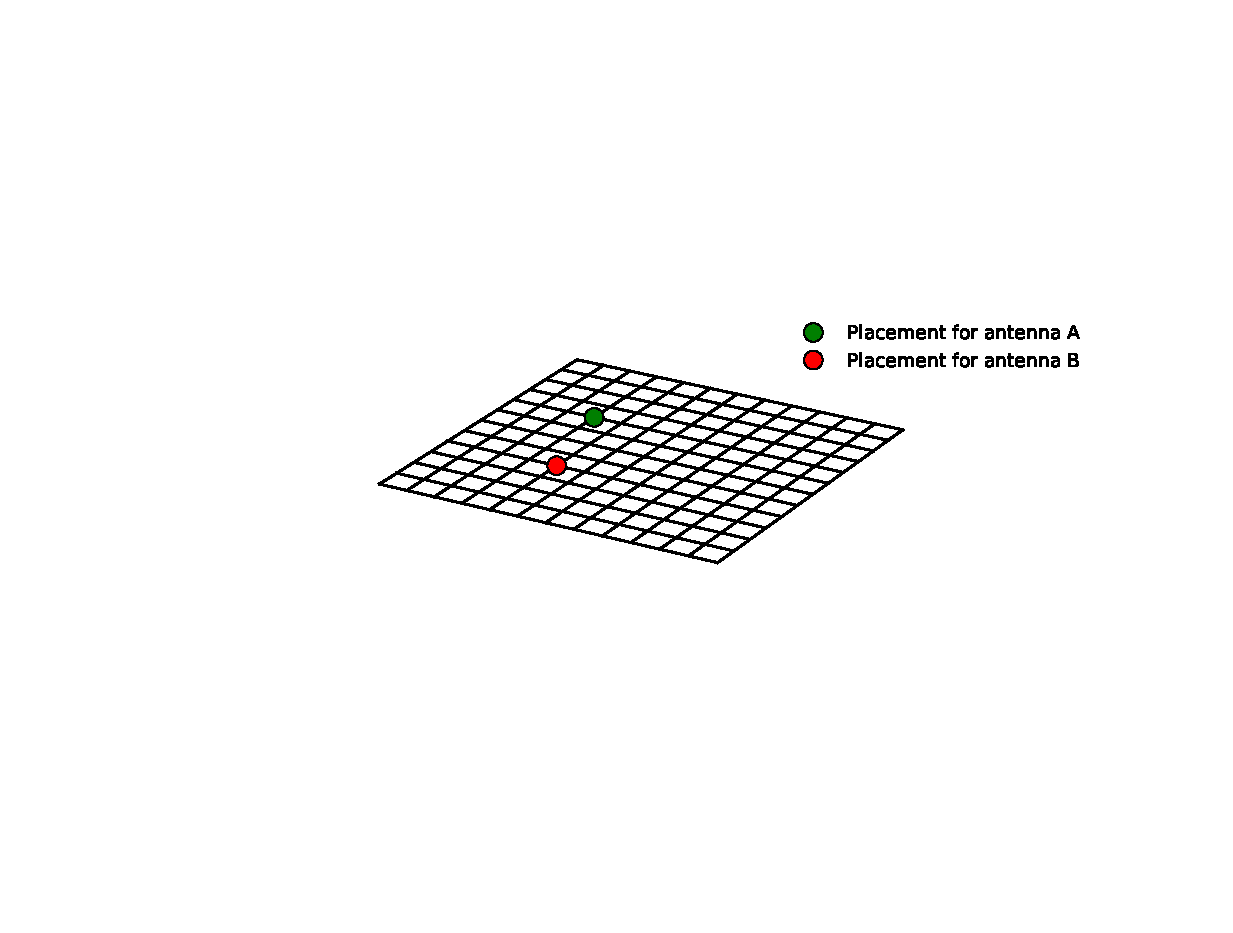
\includegraphics[trim=125 165 50 135, clip, scale=0.35]{../paper/FIG/tc1_mut3}
                }
            \end{minipage}
    \end{enumerate}
\end{frame}

\begin{frame}[t]{Stochastic Algorithms: Crossover Operator}
    \begin{enumerate}
        \item Select two individuals from population:\par
            \begin{minipage}[t]{\linewidth}
                \centering
                \adjustbox{valign=t}{%
                    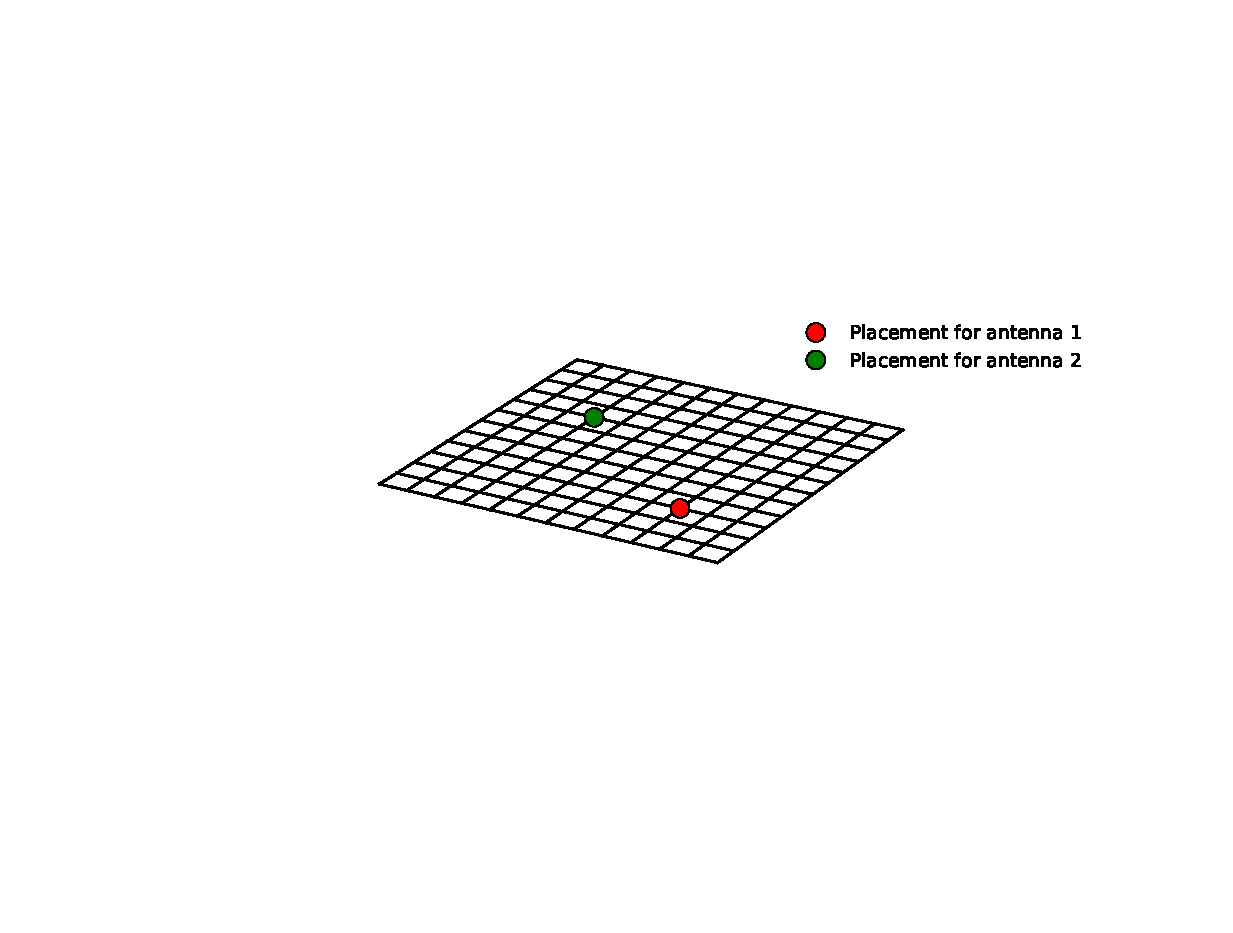
\includegraphics[trim=175 165 50 135, clip, scale=0.35]{../paper/FIG/tc1_reco1}
                    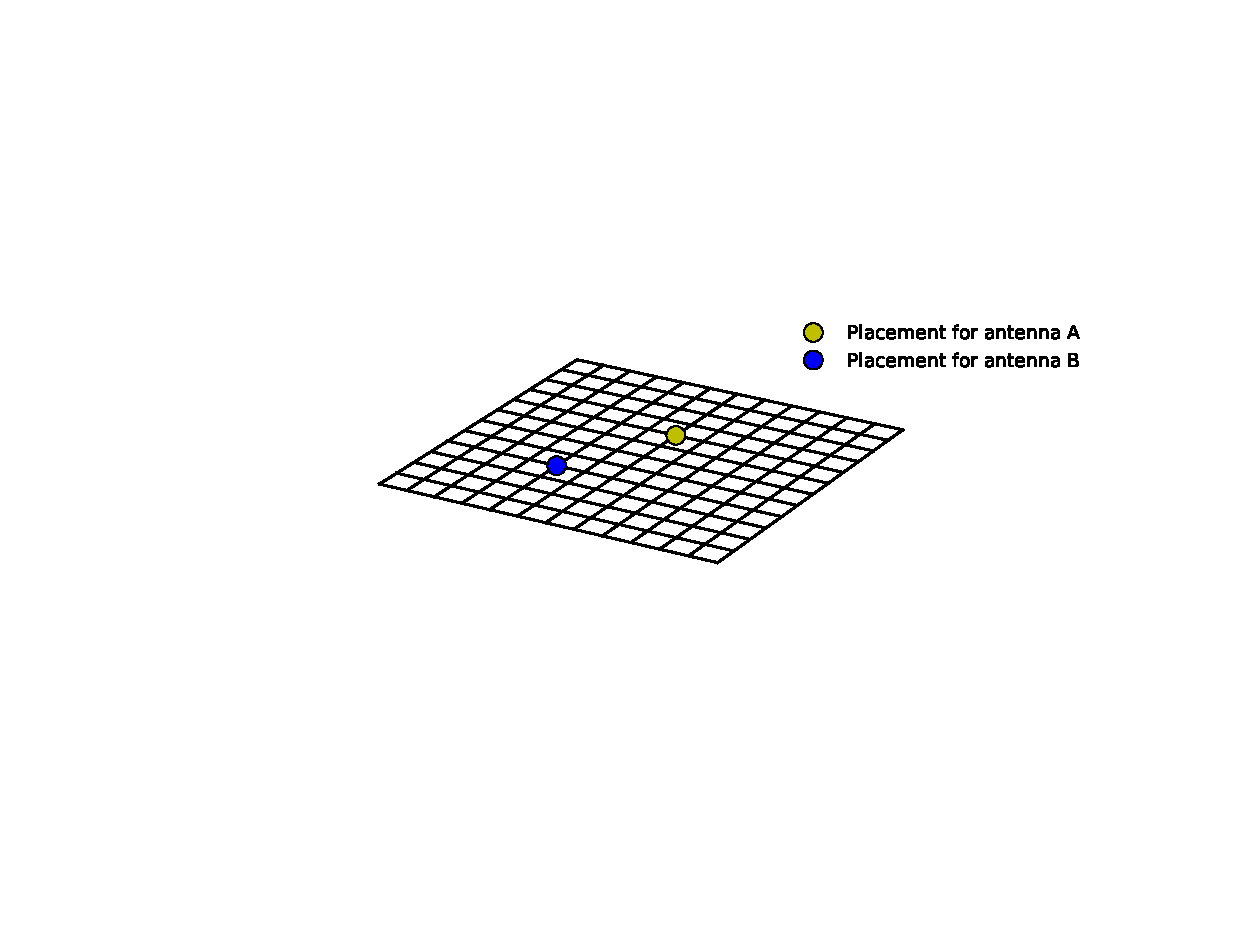
\includegraphics[trim=175 165 50 135, clip, scale=0.35]{../paper/FIG/tc1_reco2}
                }
            \end{minipage}
        \item Select a crossover point, and swap placements prior to the point: \par
            \begin{minipage}[t]{\linewidth}
                \centering
                \adjustbox{valign=t}{%
                    \begin{tabular}{ll:l}
                        $\text{ind}_1:$&$\textcolor{red}{A_1}$ & $\textcolor{drkgreen}{A_2}$ \\
                        &\makebox[\widthof{A\_1}][l]{$\downarrow$} &\\
                        $\text{ind}_2:$&$\textcolor{blue}{A_1}$ & $\textcolor{aureolin}{A_2}$ \\
                    \end{tabular}
                }
            \end{minipage}
    \item Two new offsprings created:\par
            \begin{minipage}[t]{\linewidth}
                \centering
                \adjustbox{valign=t}{%
                    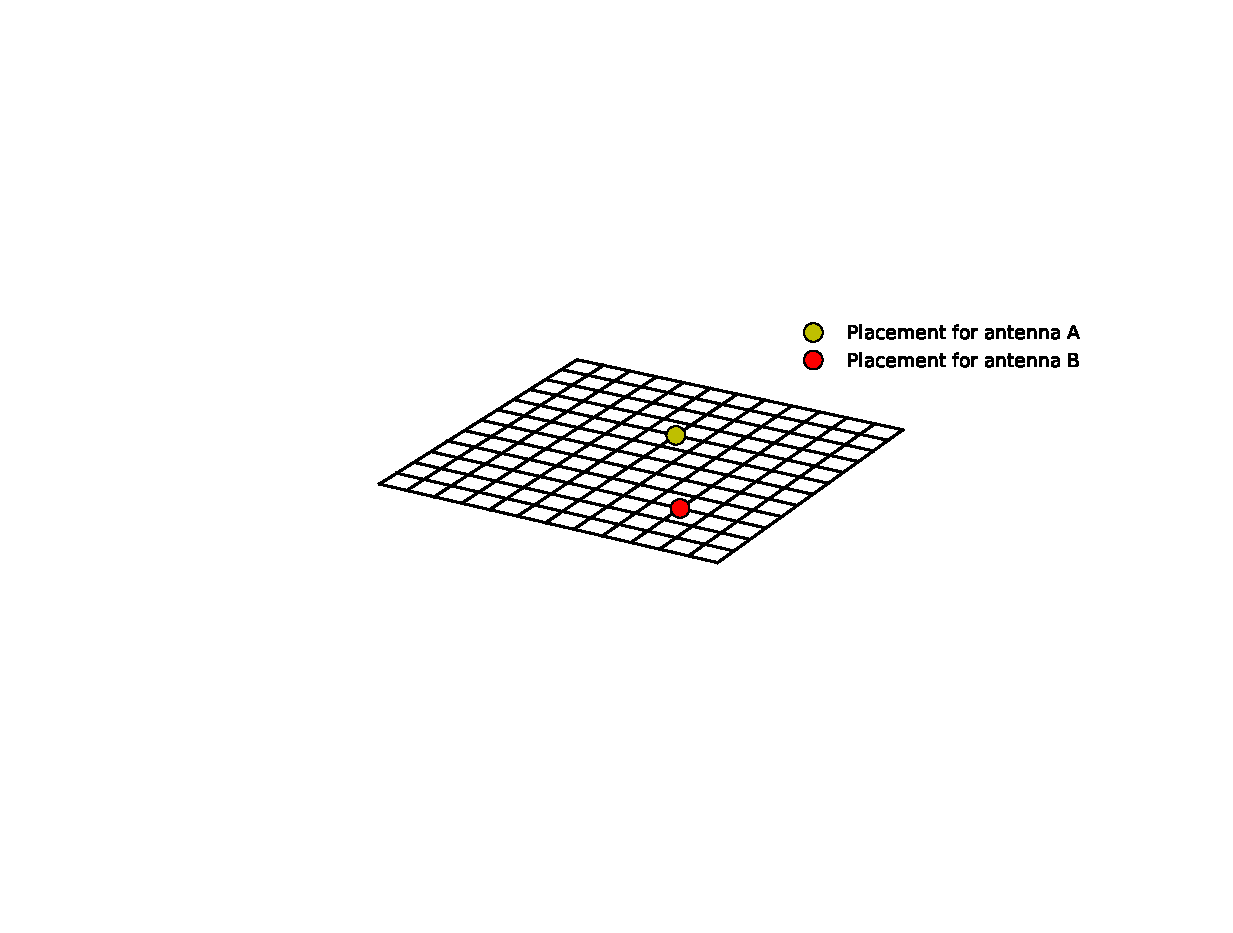
\includegraphics[trim=175 165 50 135, clip, scale=0.35]{../paper/FIG/tc1_reco3}
                    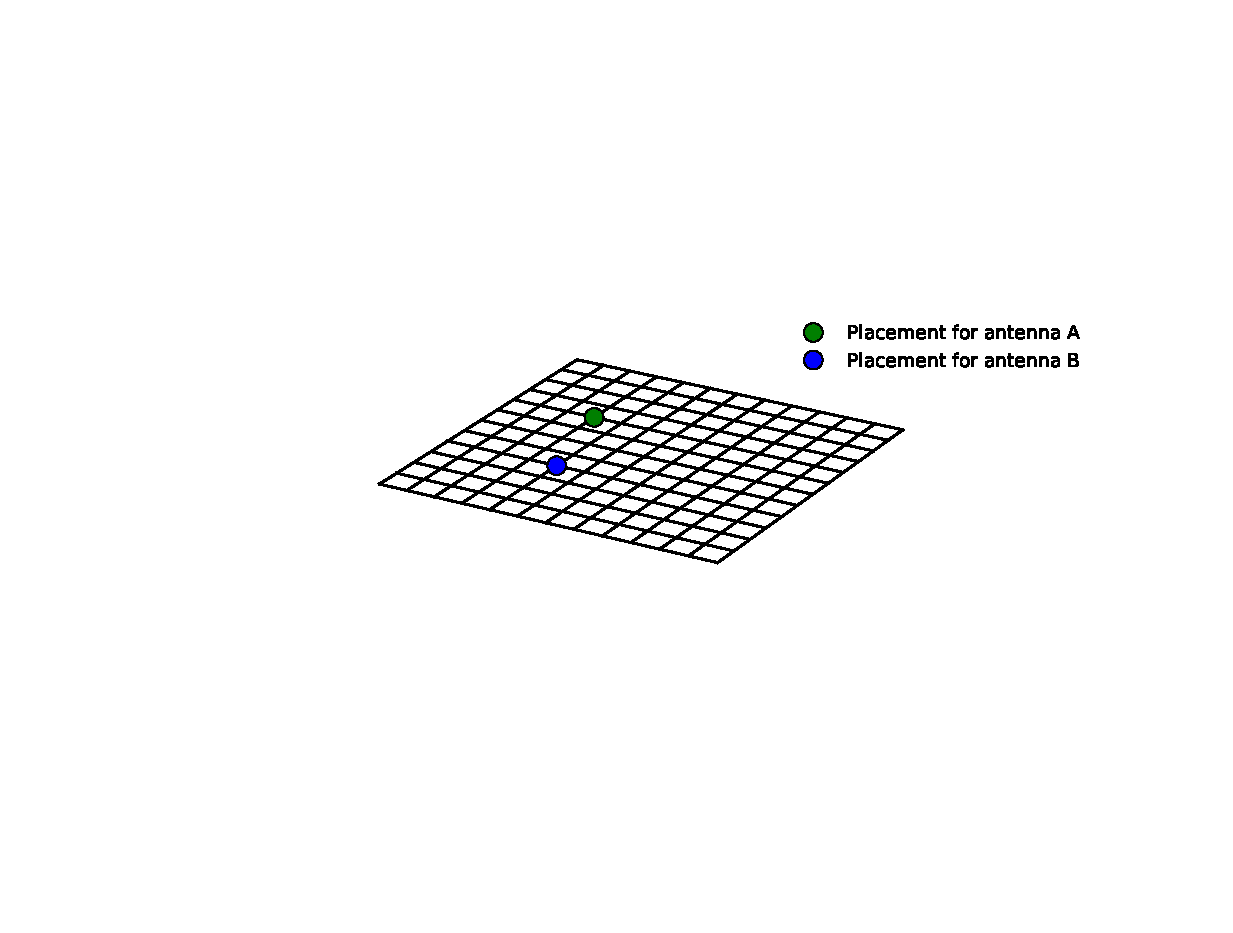
\includegraphics[trim=175 165 50 135, clip, scale=0.35]{../paper/FIG/tc1_reco4}
                }
            \end{minipage}
    \end{enumerate}
\end{frame}



\begin{frame}{Genetic Algorithm}
    \begin{spacing}{0.6}
        \fontsize{8}{12}\selectfont
        \begin{algorithm}[H]
            Initialize $P\leftarrow$ generate $p$ random individuals.
            Compute the $fitness(h_i), i \in [1,p]$, and order $P$ based on fitness\;
            $i=0$ \;
            \While{$i<gen_{max}$} {
                Elitism: Select $n_e$ fittest individuals to add to $P'$ \;
                \For{$(p - n_e)/2$ times} {
                    $M \leftarrow select(P, 2)$\;
                    \HiLi \eIf {$rand(0,1)<p_c$} {
                        Apply $crossover(M)$ to get two offsprings $O$ \;
                        Add $O$ to $P'$ \;
                    }
                    { Add $M$ to $P'$ \; }
                }
                Uniformly select $p_{m} \cdot (p - n_e)$ individuals from $P$, and apply $mutate$ operator to each \;
                Update $P\leftarrow P'$ \;
                Compute $fitness(h_i); i \in [1, p]$, and order $P$ based on fitness \;
                Update $i \leftarrow i + 1$ \;
            }
            \caption{AP-GA}
        \end{algorithm}
    \end{spacing}
\end{frame}


\begin{frame}{Evolutionary Strategy}
    \fontsize{8}{12}\selectfont
    \begin{algorithm}[H]
        Initialize $P\leftarrow$ generate $\mu$ random individuals\;
        $i=0$ \;
        \While{$i<gen_{max}$} {
            Create $\lambda / \mu$ offsprings from  each $\mu$ individuals by applying mutation operator, and add all offsprings to $P$ \;
            Compute the $fitness(h_i), i=1,\ldots, \lambda$ \;
            Keep $\mu$ best individuals in P, and discard remaining $\lambda - \mu$ individuals \;
            Update $i \leftarrow i+1$
        }
        \caption{ES}
    \end{algorithm}
\end{frame}

\begin{frame}{Simulated Annealing}
    \fontsize{8}{8}\selectfont
    \begin{algorithm}[H]
%\scriptsize
        Initialize $C\leftarrow$ generate a random individual \;
        $i=0$ \;
        \While{$i<i_m$} {
            $N \leftarrow mutate(C)$ \; 
            \eIf{$fitness(C) < fitness(N)$} {
                \If{$rand(0,1) < e^{-\delta f / T}$} {
                    $C \leftarrow N$
                }}  {
                $C \leftarrow I$ \; }
                $T \leftarrow T \cdot f_{cooling}$ \;
                $i \leftarrow i + 1$ \;
            } 
            \caption{SA}
            \label{alg:ap-sa}
        \end{algorithm}
    \end{frame}


    \begin{frame}[t]{Experimental Setup}
        \begin{enumerate}
            \item Create (s) such that each individual is defined by a placement for each of the $m$ antennas
            \item Run all individuals through \textit{NEC} simulator \footnote{http://www.nec2.org} to get fitness parameters 
            \item Apply EA operators 
            \item Repeat till either global minimum is reached or 50\% evaluations of search space 
        \end{enumerate}
        \vspace{10mm}
    \end{frame}

    \begin{frame}{Experiments: Test Cases}
        \begin{figure}
            \centering
            \begin{subfigure}{.5\columnwidth}
                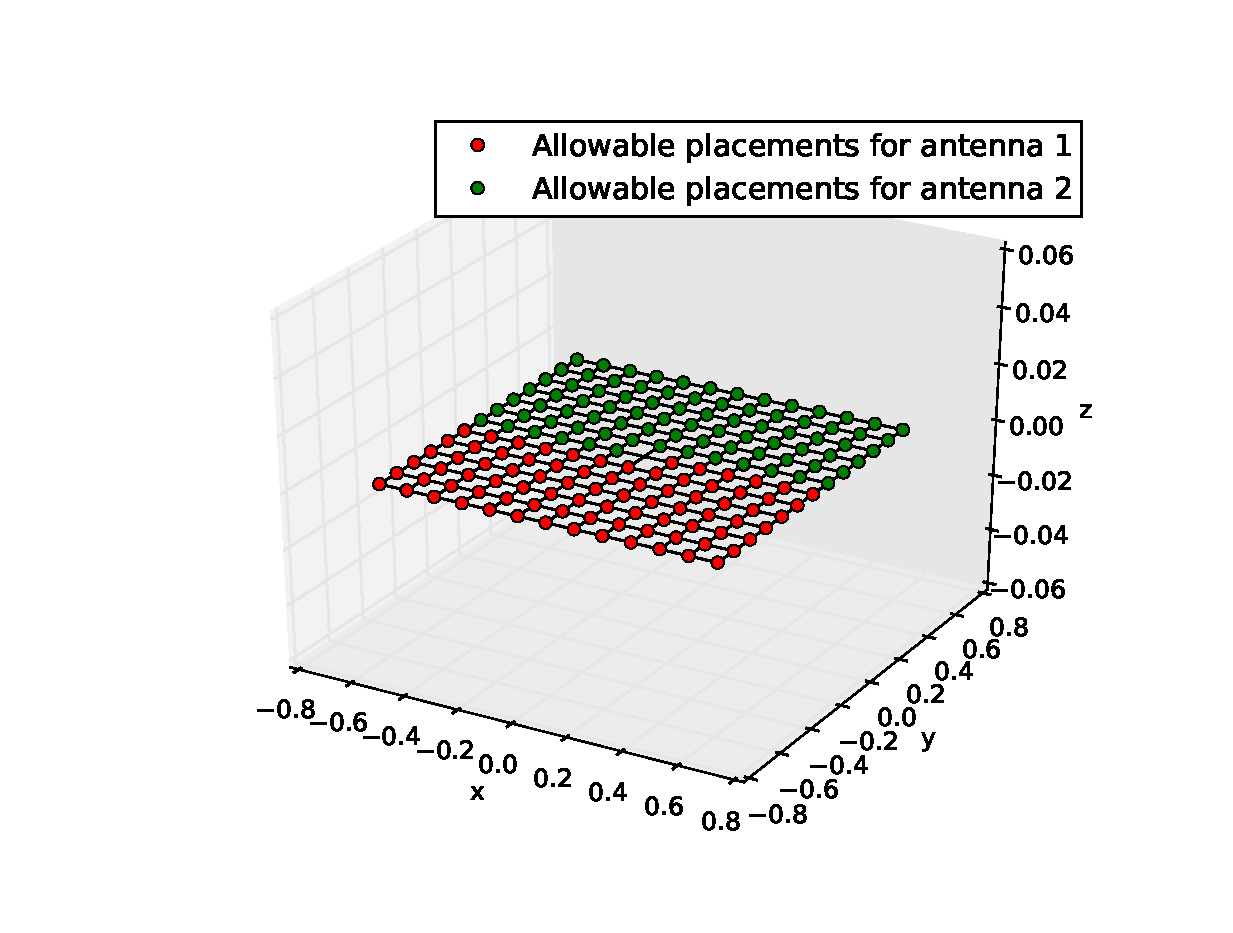
\includegraphics[width=\columnwidth,height=\columnwidth]{../paper/FIG/tc_1_figure}%
                \caption{\tiny Test Case 1 with $7056 (83x83)$ allowable placements}%
                \label{fig:tc1_figure}%
            \end{subfigure}\hfill%
            \begin{subfigure}{.5\columnwidth}
                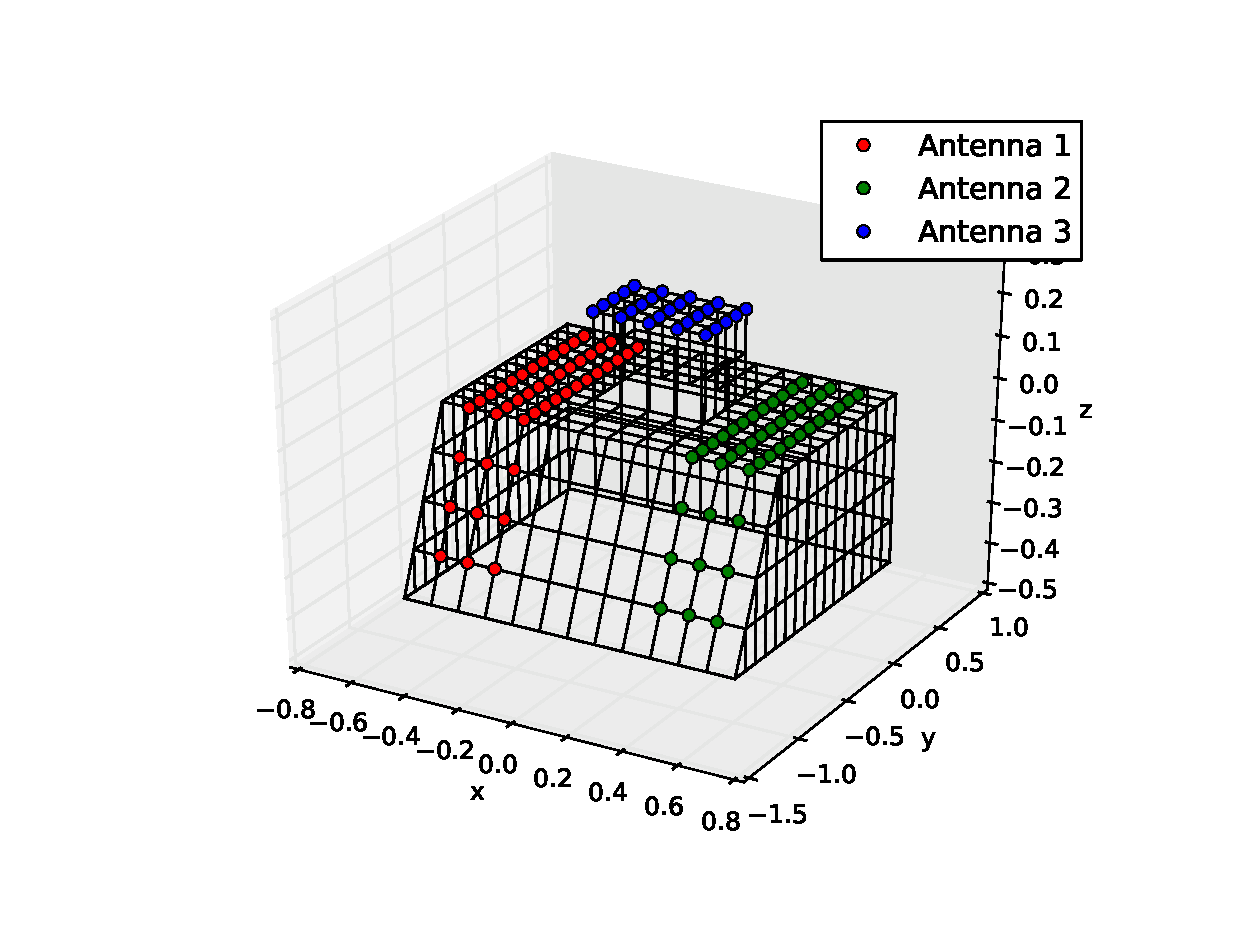
\includegraphics[width=\columnwidth, height=\columnwidth]{../paper/FIG/tc_2_figure}%
                \caption{\tiny Test Case 2 with $50625 (45x45x45)$ allowable placements}%
                \label{fig:tc2_figure}%
            \end{subfigure}\hfill\\%
        \end{figure}
    \end{frame}

    \begin{frame}{Experiments: Test Cases}
        \begin{figure}
            \centering
            \begin{subfigure}{.5\columnwidth}
                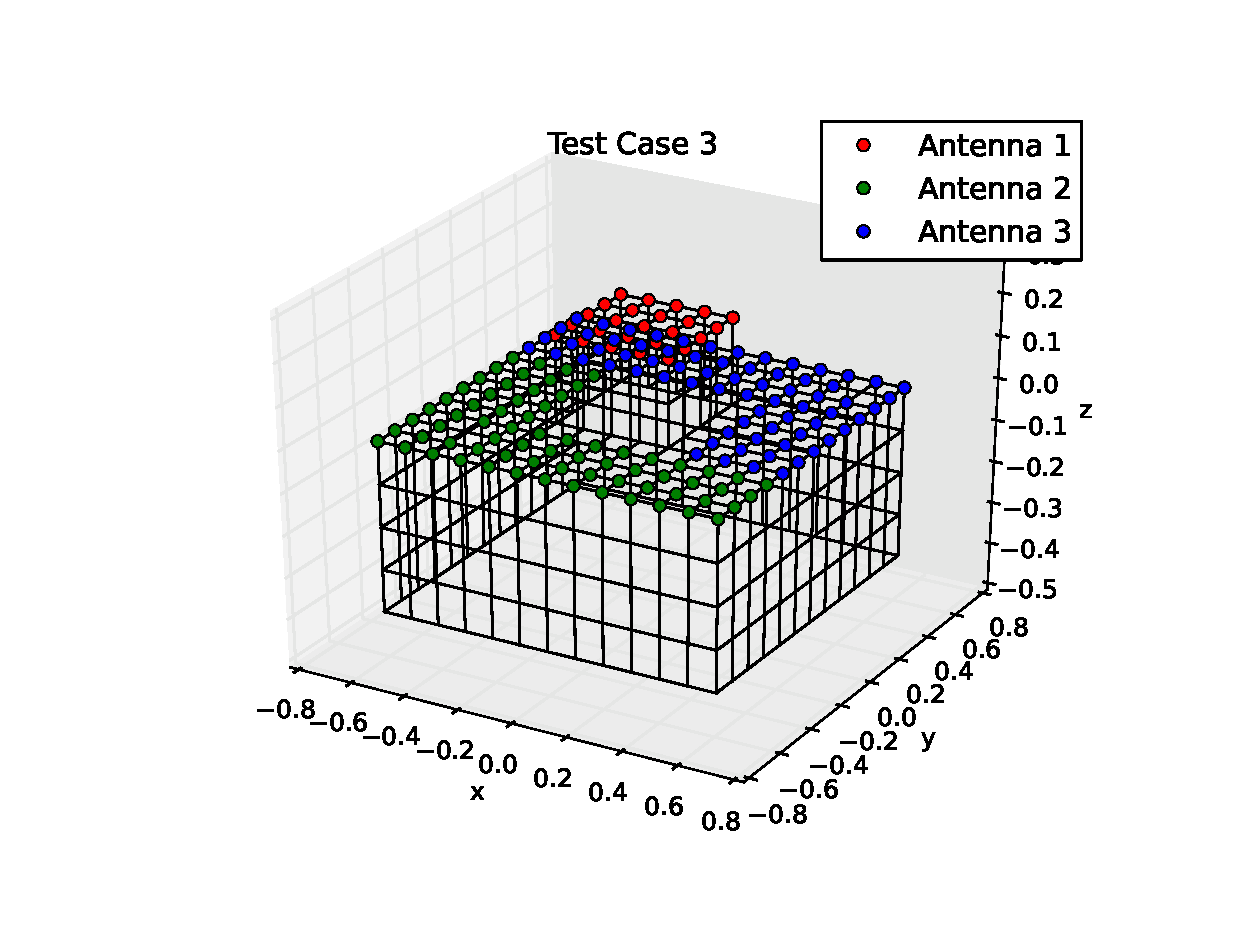
\includegraphics[width=\columnwidth,height=\columnwidth]{../paper/FIG/tc_3_figure}%
                \caption{\tiny Test Case 3 with $126025 (71x71x25)$ allowable placements}%
                \label{fig:tc3_figure}%
            \end{subfigure}\hfill%
            \begin{subfigure}{.5\columnwidth}
                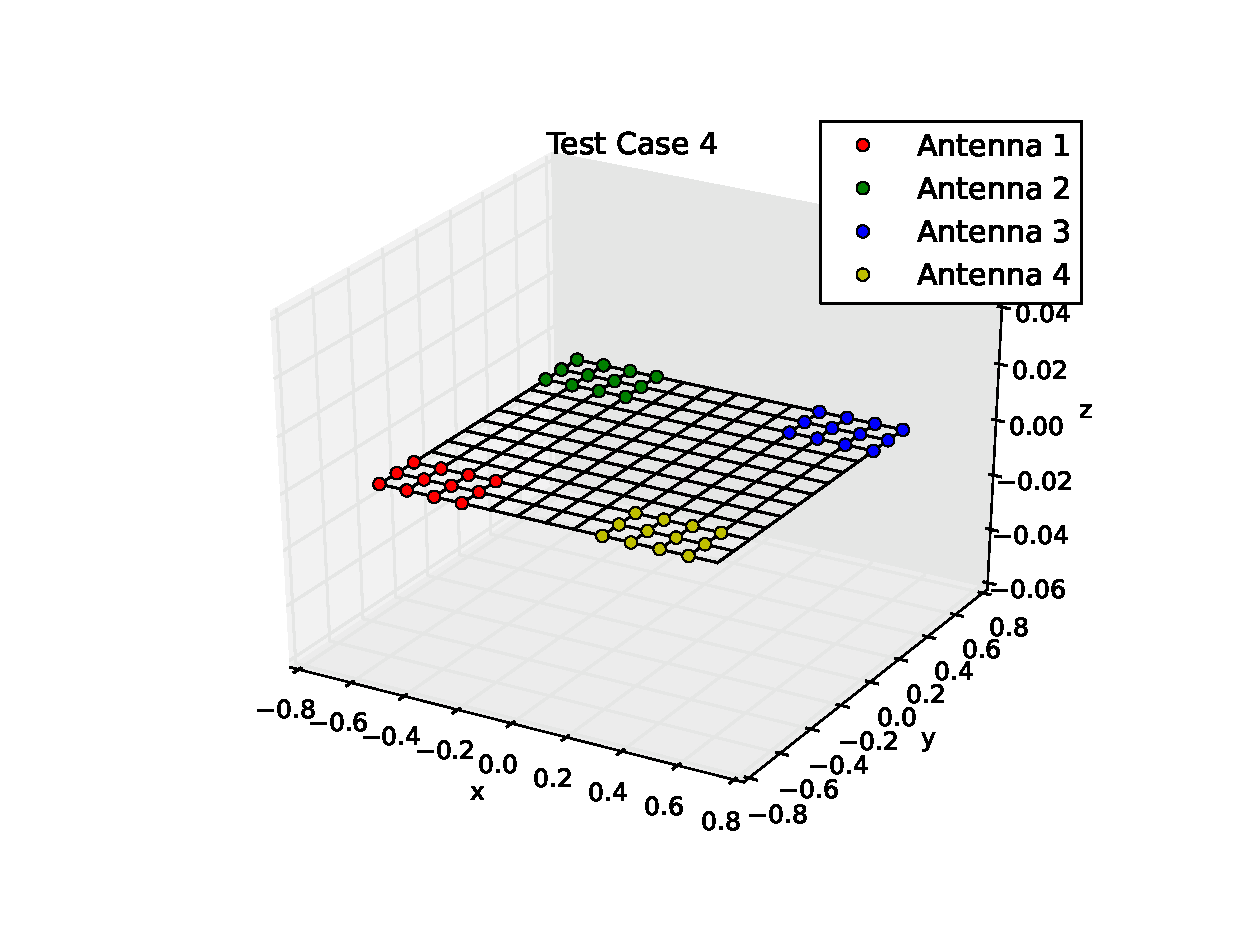
\includegraphics[width=\columnwidth, height=\columnwidth]{../paper/FIG/tc_4_figure}%
                \caption{\tiny Test Case 4 with $20736 (12x12x12x12)$ allowable placements}%
                \label{fig:tc4_figure}%
            \end{subfigure}\hfill\\%
        \end{figure}
    \end{frame}

    \begin{frame}{Results}
        \begin{center}
            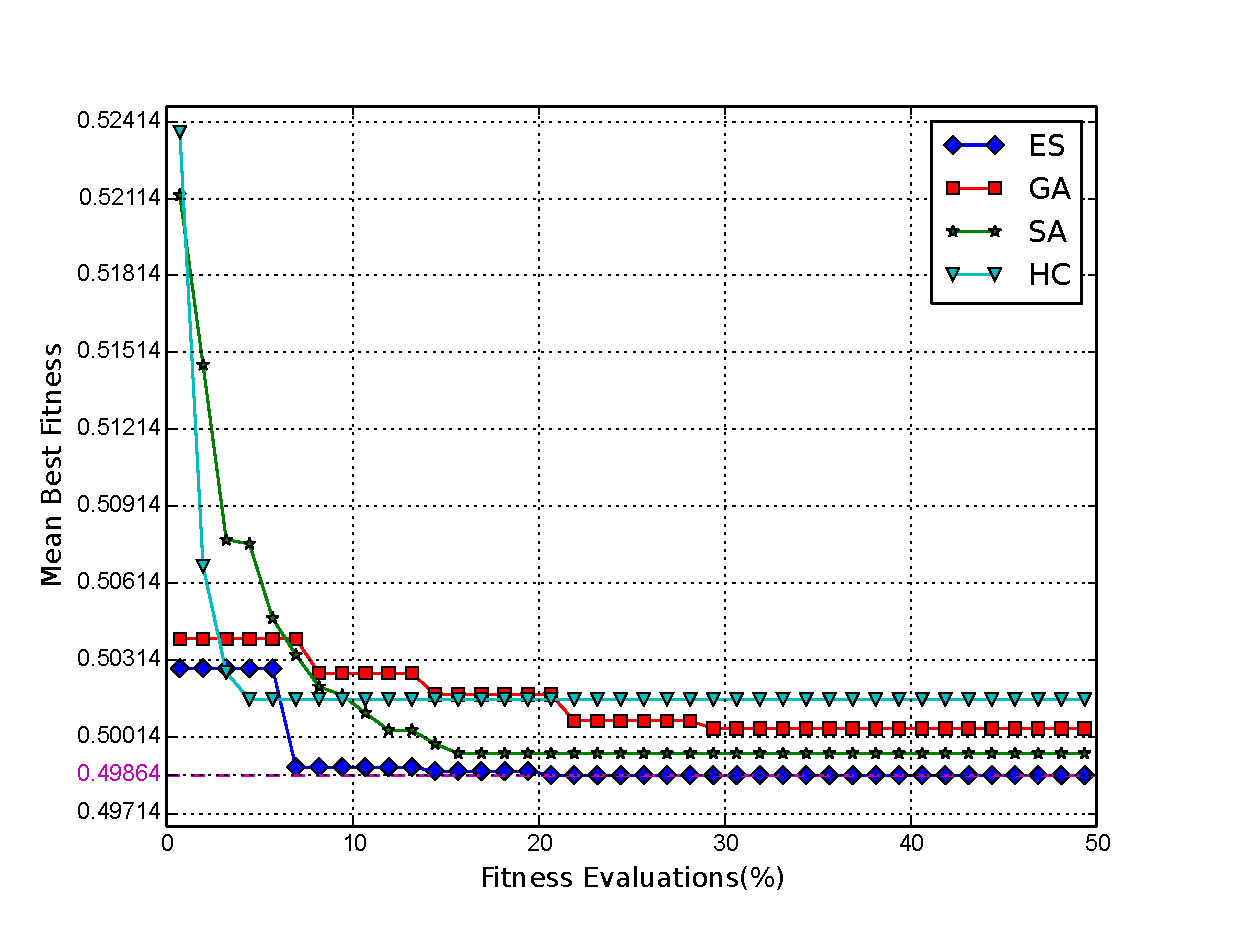
\includegraphics[width=.49\textwidth]{../paper/FIG/tc1_mf.eps}
            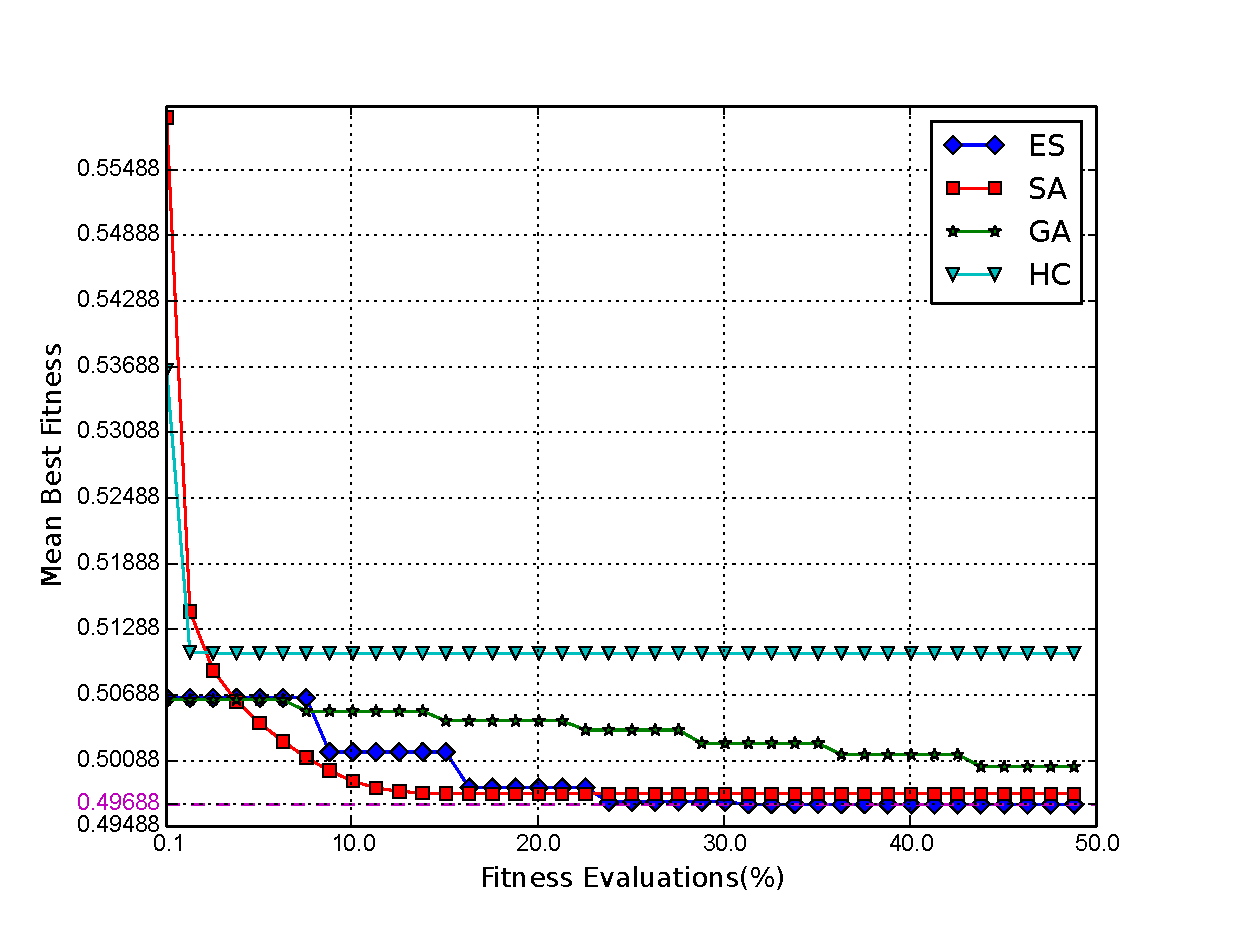
\includegraphics[width=.49\textwidth]{../paper/FIG/tc2_mf.eps}
        \end{center}
    \end{frame}

    \begin{frame}{Results}
        \begin{center}
            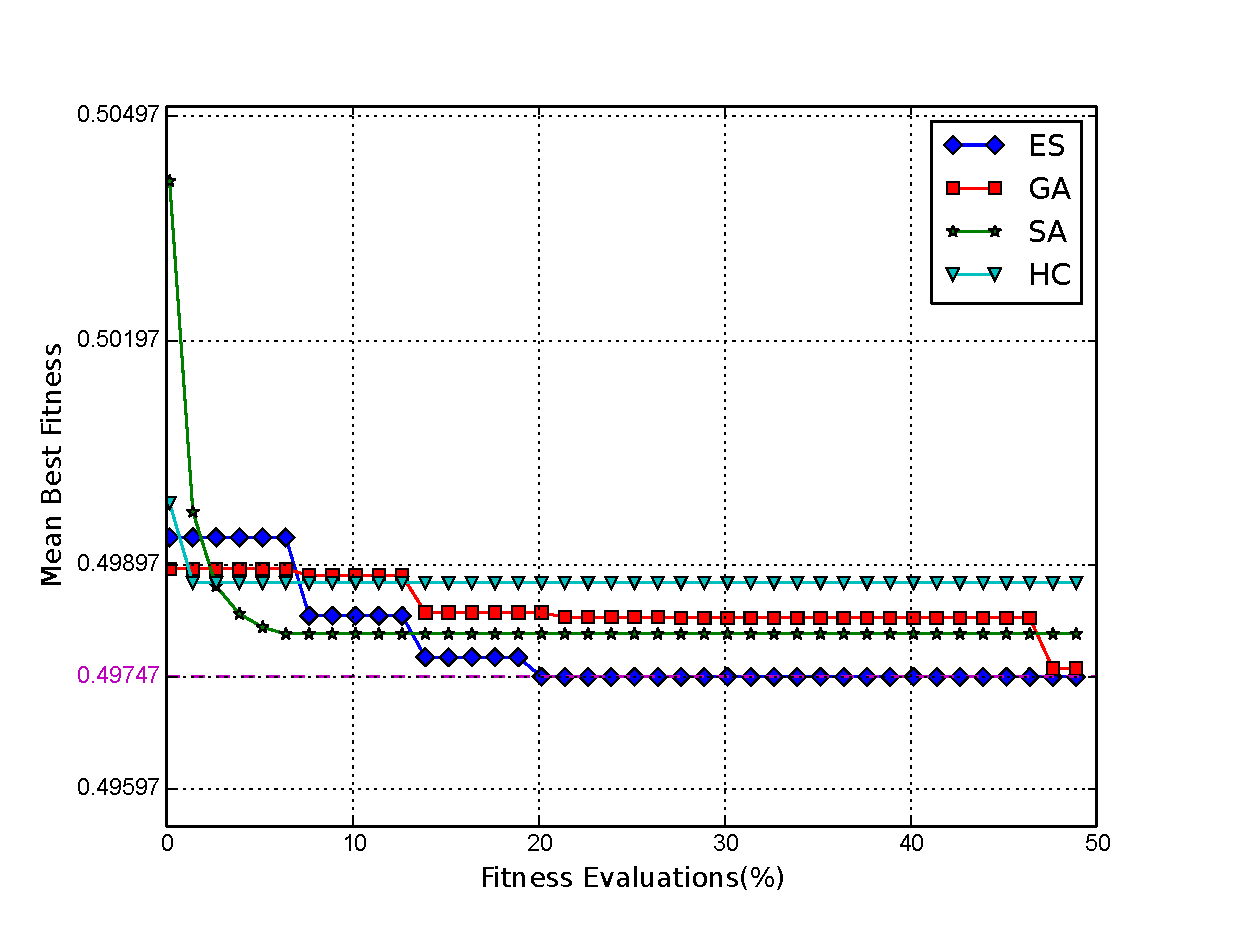
\includegraphics[width=.49\textwidth]{../paper/FIG/tc3_mf.eps}
            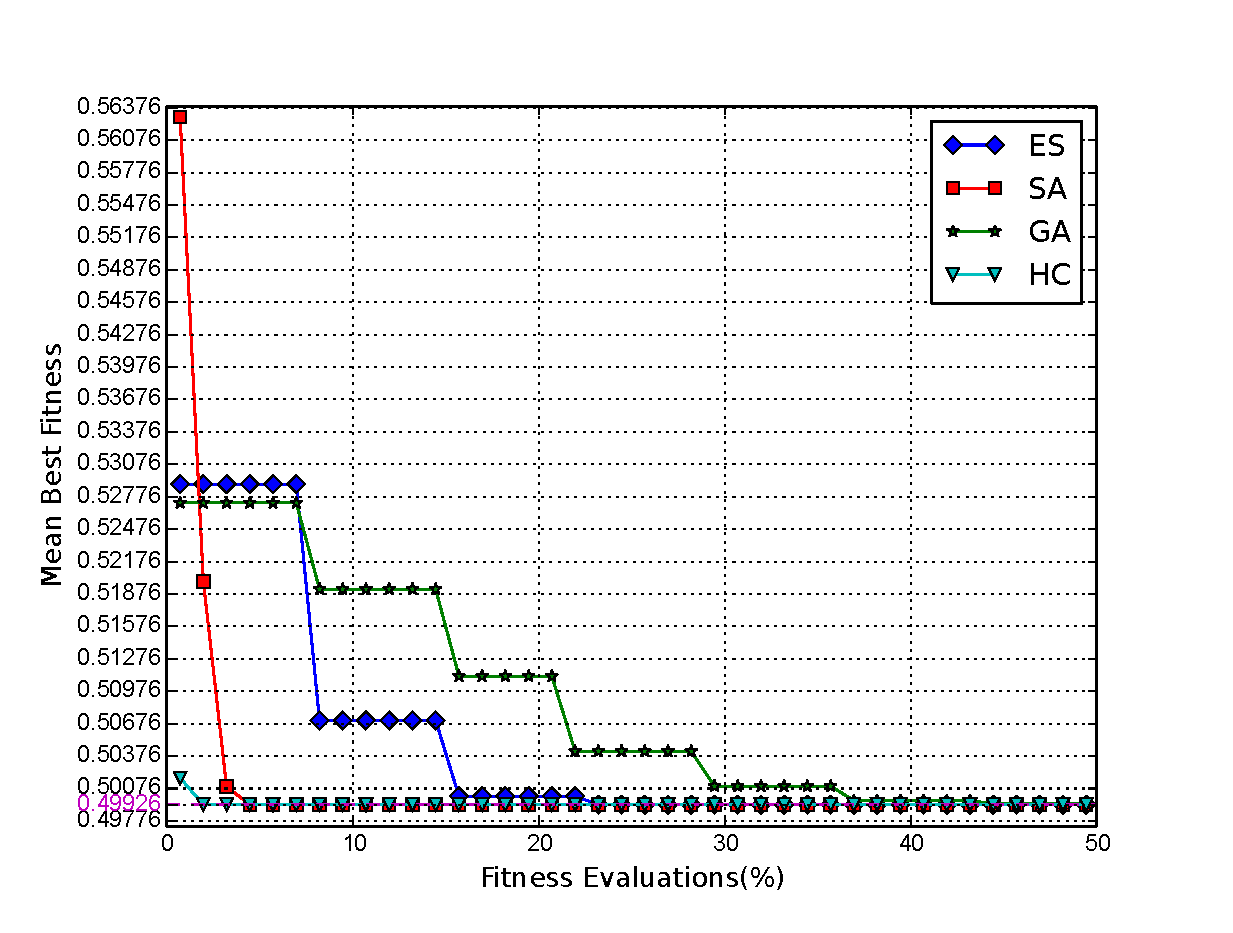
\includegraphics[width=.49\textwidth]{../paper/FIG/tc4_mf.eps}
        \end{center}
    \end{frame}

    \begin{frame}{Equivalence of fitness to efficiency}
        \small For a particular test case, fitness change of $0.01$ is equivalent to either the corresponding value under expected gain ($\mathbb E_g$) column, or difference in coupling ($\Delta_c$).
        \begin{table}
            \centering
            \begin{threeparttable}
                \begin{tabular}{|C{1cm}|C{2.5cm}|C{2.5cm}|} \hline
                    ID& $\mathbb E_g$ & $\Delta_{c}$ (dB) \\ \hline
                    tc1 & 872.277 & 0.5474 \\ \hline
                    tc2 & 862.082 & 1.3034 \\ \hline
                    tc3 & 861.845 & 1.5180 \\ \hline
                    tc4 & 871.049 & 0.5693 \\
                    \hline\end{tabular}
            \end{threeparttable}
        \end{table}
        \tiny
        $\mathbb E_g = \frac{1}{N \cdot m} \sum_{i}^m F_{RP}(A_i),$
        where $N = \;\mid \theta \mid \cdot \mid \phi \mid$
    \end{frame}

    \begin{frame}{Conclusion}
        \begin{itemize}
            \item Formulation of the antenna placement problem
            \item Generic problem formulation to accommodate multiple antennas and platforms
            \item Optimal placements found using stochastic algorithms
        \end{itemize}
    \end{frame}

    \end{document}
